\documentclass[12pt, letterpaper]{article}
\usepackage{graphicx}
\usepackage{hyperref}
\usepackage{mathtools}
\begin{document}
\title{Color Model Composition}
\author{Joshua Gang}
\date{\today}
\maketitle

\section{Introduction}

\paragraph{} We have models, represented by $\theta(\text{name})$, which are sets of parameters describing a specified color. These models are derived from Randal Monroe's Color Survey data. All of these models are contained within LUX, a system designed by Brian MacMahan. Within the lexicon there exist color labels that are compositions of other labels, such as 'green' and 'blue' combining to create 'green-blue'. These color compositions are currently all stated within the lexicon. If we can derive a composition function, $f(\theta(x), \theta(y)) = \theta'(x,y)$, then we can simplify the LUX lexicon by removing the composed colors, thus reducing the number of parameters. 

\paragraph{} There are a few steps that are required in order to determine what this composition function is. The first step is an evaluation metric in order to determine whether or not two $\theta$s are the same. Afterwards, we can construct a composition function and test how well it does. Preliminary work also shows us a special case of composition functions, that will be discussed later.

\section{Twins}

\paragraph{} In order for us to determine whether or not our $f$ is generating a $\theta$ that is comparable to the one already present within LUX, we must first find a baseline for $\theta$s  in LUX that should already be identical. Within LUX, there exist $\theta$s, called "twins", where both $\theta(x,y)$ and $\theta(y, x)$ exist. We propose that these two $\theta$ are the same, namely that $\theta(x,y) == \theta(y, x)$. If that is true, then we can use the same evaluation metric on $\theta'$s when comparing them to $\theta$s, and that will tell us whether or not the two are the same. 

\begin{figure}[h]
\begin{center}
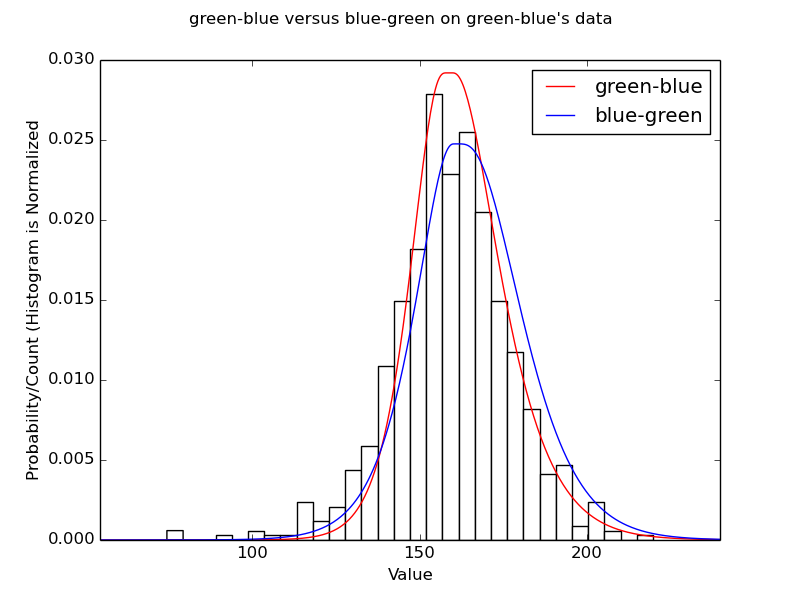
\includegraphics[width=.75\textwidth]{green-blue}
\end{center}
\caption{An example of a twin, Blue-Green and Green-Blue. They are both distributions that are very similar to each other, as you can see by their positions relative to the data for green-blue.}
\label{fig:twin_blue_green}
\end{figure}

\paragraph{} The evaluation metrics that can be used can either be $r^2$ or log-likelihood values, both being used on the other twin's data set. The same metric would then be applied to the $\theta'$, and would give us an idea of how accurate they are. Preliminary results using $r^2$ on the twins tells us that on average, the twins have a $r^2$ metric of .76. More can be seen in \autoref{app:r2_values}

\paragraph{} Figuring out what the evaulation metric result for the twins, to be used for the composition function $f$, doesn't actually tell us if they are the same. Rather it tells us if they are the same, then what the metrics will tell us. In order to determine whether or not they are the same, we believe that a survey needs to be conducted on each of the twins. By having people rate on a scale of 1-10 how close two colors are to each other, we can get a human perspective on which colors are the same. The twins should all have very high values, averaging anywhere from 7-10, whereas non-twin colors should have significantly lower values, averaging anywhere from 1-4. If so, then we can say with high confidence that the twins are the same, and that $\theta(x,y) == \theta(y, x)$, which then means that we can use the evaluation metrics to compare other distributions.

\section{Composition $f$}

\paragraph{} Once we determine an evaluation metric, then we can create the composition function $f$. $f$ should probably be a machine learning regressor, in the hopes that such a machine will be able to determine relationships between different parameters in the model that might not be otherwise obvious.

\paragraph{} There are many ways to structure the inputs into $f$. Every one of the $\theta$s has a property $\phi$, or availability, which states how "popular" the $\theta$ is. One way of ordering the inputs into $f$ would be to organize them by availability, under the assumption that the more popular a $\theta$ is, the larger of an impact it has on the resulting $\theta'$. Another way is to organize the inputs by their order in $\theta'$'s name, under the assumption that the order implies some significance in which $\theta$ is more impactful in the composition to produce $\theta'$. The final, and most intuitive  ordering, is to order the $\theta$s by their relative positions on the color wheel, under the assumption that the mix of colors is more towards an average of the two $\theta$s than anything else. Such an ordering would allow for the easiest discovery of such a fact.

\paragraph{} Have to talk about hue adjust first before running the trees.

\section{Special Cases of $f$, Noun-Colors}

\paragraph{} Colors can be named almost anything. Often times, there are nouns, objects that are present in the physical world, that we use to describe what a color looks like. That color is so ingrained with the identity of the object that it is understood what that color looks like, just by calling it by it's real-world counterpart. These colors are shades of other colors in the lexicon, such as "chocolate" being a shade of "brown". What happens when you combine the two colors? What is the real difference between "brown" and "chocolate brown"? As one is a shade of the other, it doesn't make sense to use the same Composition $f$ that we did before in this case.

\paragraph{} These Noun-Colors are not equivalent to the base Nouns. Using the $r^2$ metric as we did above, we come out with only 0.31307, well below the Twin's $r^2$ value of .76. For other comparison purposes, we can approximate Gaussean distributions of the colors by generating them with the raw data. Doing so allows us to easily compare different characteristics of the distributions, such as their position on the color spectrum or how much wider one is than the other.
\begin{figure}[h]
\begin{center}
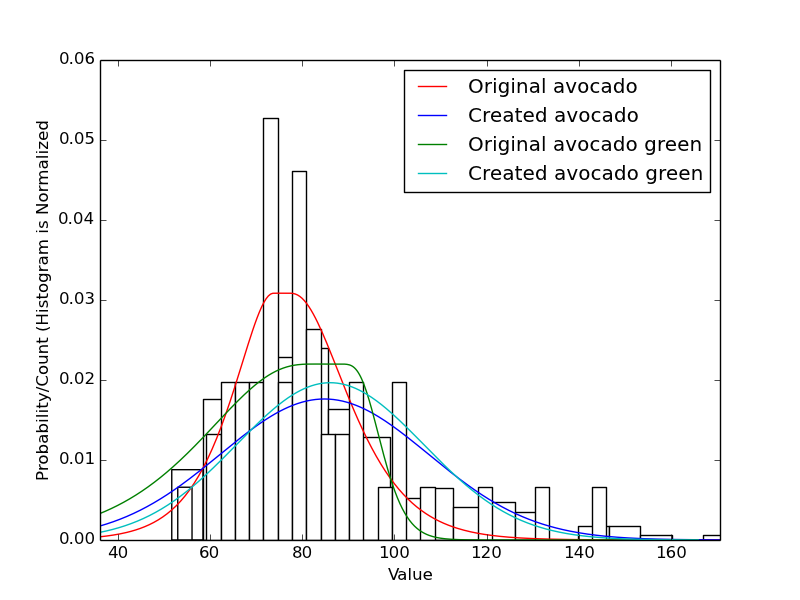
\includegraphics[width=.75\textwidth]{gaussean_differences}
\end{center}
\label{fig:gauss_diff_avocado}
\caption{An example showing how the gausseans can be used to compare. I don't think that this actually works though, because the original avocado is skinnier than the original avocado green, but the created (gaussean) avocado is fatter than the created avocado green}
\end{figure}While using this, in general, the Noun + Color distributions tended to be wider than the purely Noun distributions, which would suggest that |something something something, need to figure out how to show that the data says this is acting weirdly. I think that it's what it's saying|.%have to put mean graph here
\begin{figure}[h]
\begin{center}
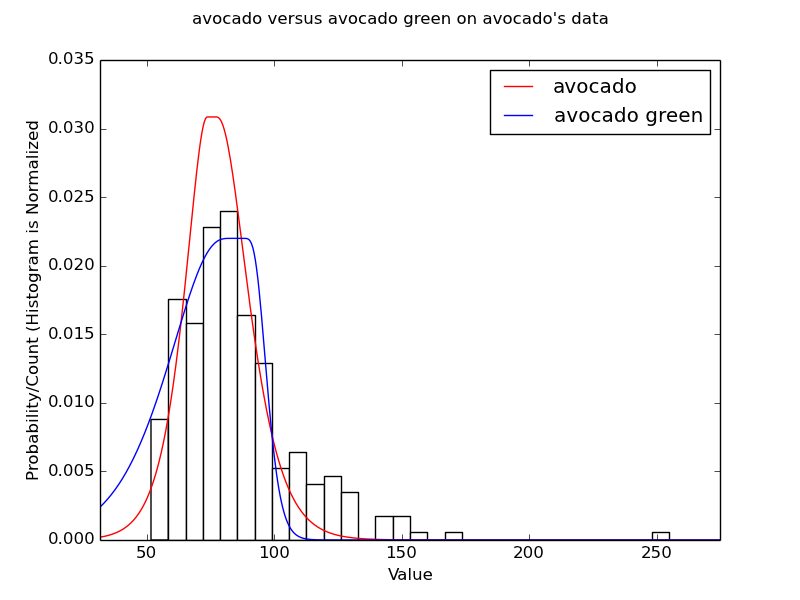
\includegraphics[width=.75\textwidth]{avocado}
\end{center}
\caption{Avocado and Avocado Green. Avocado Green appears to be wider than Avocado, suggesting that when people use it, they are describing a broader range of color than just with Avocado.}
\label{fig:avocado}
\end{figure}


\pagebreak
\appendix{}
Appendix
\section{Twins $r^2$ Values}
\label{app:r2_values}
\paragraph{}All values are the $ r^2$ values for the X model on the Y's data points.
\begin{center}
\begin{tabular}{| l | l | c | c |} \hline
First Color & Second Color & First on Second & Second on First \\ \hline
green-grey & grey green & 0.909311 & 0.921990 \\ \hline
grey-brown & brown-grey & 0.541379 & 0.784039 \\ \hline
red-brown & brown-red & 0.875762 & 0.838473 \\ \hline
purple-pink & pink-purple & 0.756994 & 0.841505 \\ \hline
red-pink & pink-red & 0.902846 & 0.904270 \\ \hline
orange-red & red-orange & 0.934824 & 0.945147 \\ \hline
blue-green & green-blue & 0.680046 & 0.817502 \\ \hline
green-brown & brown-green & 0.891857 & 0.837641 \\ \hline
purple blue & blue-purple & 0.955867 & 0.943420 \\ \hline
blue-grey & grey blue & 0.923963 & 0.912297 \\ \hline
violet red & red violet & 0.719531 & 0.459585 \\ \hline
yellow-brown & brown yellow & 0.575357 & 0.781066 \\ \hline
yellow-orange & orange-yellow & 0.470531 & 0.788876 \\ \hline
red-purple & purple-red & -0.408986 & 0.511436 \\ \hline
violet blue & blue violet & 0.789110 & 0.622474 \\ \hline
grey purple & purple grey & 0.851877 & 0.901247 \\ \hline
orange-brown & brown-orange & 0.512578 & 0.787795 \\ \hline
green-yellow & yellow-green & 0.955530 & 0.949561 \\ \hline
\end{tabular}
\end{center}
\paragraph{} The average is 0.760741727251.

\end{document}